\section{Context}%\fxfatal{Kan godt v�re det ikke skal hedde context}
%Hvad laves projektet som
%Noget med proof of concept

The project will be developed as if it was a service offered by a company.
Therefore the system, known as \acs{LONE}, must be developed as if it was to surveil several locations simultaneously.
%Therefore the system is to be developed as if surveillance is to be done at several locations simultaneously.
The hardware available is an AR Drone 2.0 Parrot, see Figure~\ref{fig:pic_of_drone}.
%The hardware available limits the project is of limited quality and the number of drones is limited too.
It is not possible to develop a system usable in the real world using this hardware.
This means the system will be developed to be a proof of concept.% and must be able to surveil several locations simultaneously.

%http://guide-images.ifixit.net/igi/cI6EGVSLLjjDFATI.medium
\begin{figure}[htb]
    \centering
    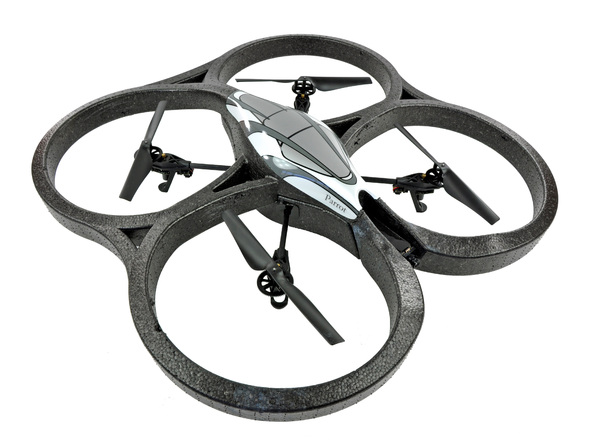
\includegraphics[width=\textwidth]{gfx/drone.jpg}
    \caption{AR Drone 2.0 Parrot.}% Picture from: http://guide-images.ifixit.net/igi/cI6EGVSLLjjDFATI.medium}
    \label{fig:pic_of_drone}
\end{figure}
